\section{Video Compression}

One of the main concepts of video compression is that while the human visual system is specifically sensitive to motion, some distortions are not as perceivable as in static images. Visual perception is limited to $<24$Hz, but flicker can be perceived up to $>60$Hz. \medskip

\textbf{Bloch's Law} \smallskip

Up to a time frame of 100ms, it does not matter "how" light arrives only the sum, e.g. 10ms of double the intensity is equal to 20ms at the normal intensity.


\subsection{Video Format}

A video sequence is a bunch of images aligned in a time sequence. The interlaced video format uses two temporal shifted half images and increases the frequency from $25$Hz to $50$Hz. 
\begin{center}
	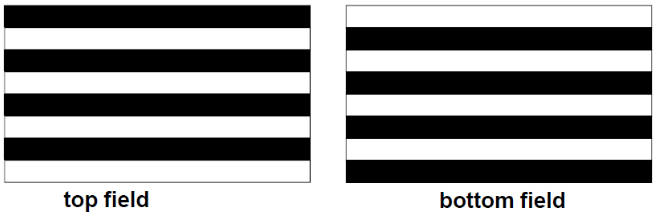
\includegraphics[width=\linewidth]{interlaced.png}
\end{center}

Today this is not done anymore, we rather use a progressive format that updates the whole screen at a time.


\subsection{Temporal Redundancy}

One way of compressing video is to take advantage of similarity between successive frames. Especially for high frame rates this works well. \medskip

The most used representation along the temporal dimension are predictive methods. There we define tree typed of frames:
\begin{itemize}
	\item \textbf{I Frame}: Intra-coded frame, independent of all other frames
	\item \textbf{P Frame}: Predictively-coded frame, based on the previous I and P frame
	\item \textbf{B Frame}: Bi-directionally predicted frame, based on both the previous and future I and P frames
\end{itemize}
\begin{center}
	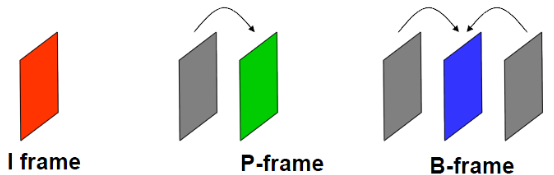
\includegraphics[width=\linewidth]{temporal_frames.png}
\end{center}

P frames can send motion vector plus changes. The frames starting at an I frame until the next I frame is also called a group of pictures (GOP). Temporal redundancy becomes inefficient if there are many scene changes or there is a lot of motion, e.g. \href{https://www.youtube.com/watch?v=r6Rp-uo6HmI&feature=youtu.be}{confetti}.

\subsubsection{Motion-Compensation Prediction}

One possibility of dealing with a high amount of motion is to use MC-prediction. Ideally we would partition the video into moving objects and describe these object motions. In reality this is very difficult, therefore we partition each frame into blocks, e.g. $16$x$16$ pixels, and try to describe the motion of each block.
\begin{center}
	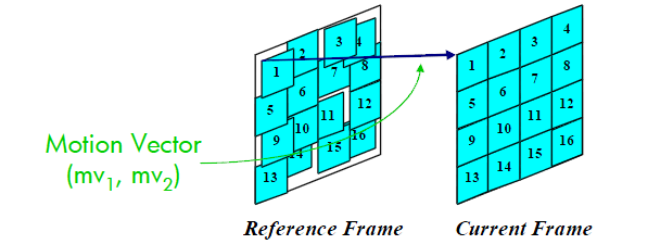
\includegraphics[width=\linewidth]{mc_prediction.png}
\end{center}

The algorithm first divides the frames into blocks and then uses the best matching blocks of the reference frame as prediction of the blocks in the current frame. For the block matching we use some best match metric, e.g. mean squared error or mean average error. The candidate blocks for the best match can either be determined by looking at all blocks or select a subset by some assumptions. \medskip

If we combine all the motion vectors, we end up with a \textbf{motion field} for all the blocks. As motion is not limited to integer-pixel offsets, one could try to estimate sub-pixel motion by spatial interpolation of the frames. The model of MC-prediction does not work well for more complex motions and might produce blocking artifacts.


\subsubsection{Bidirectional MC Prediction}

Instead of only looking at the previous frame we also take a look at the next frame. Bidirectional MC-prediction then estimates the position of a block in the current frame from either the previous frame, the next frame or the average of the previous and next frame.


\subsection{Video Compression Architecture}

Basic video compression architectures use temporal, spatial and color redundancies. Spatial redundancy uses DCT on the blocks and color redundancy does a color space conversion. A basic encoder could look as follows:
\begin{center}
	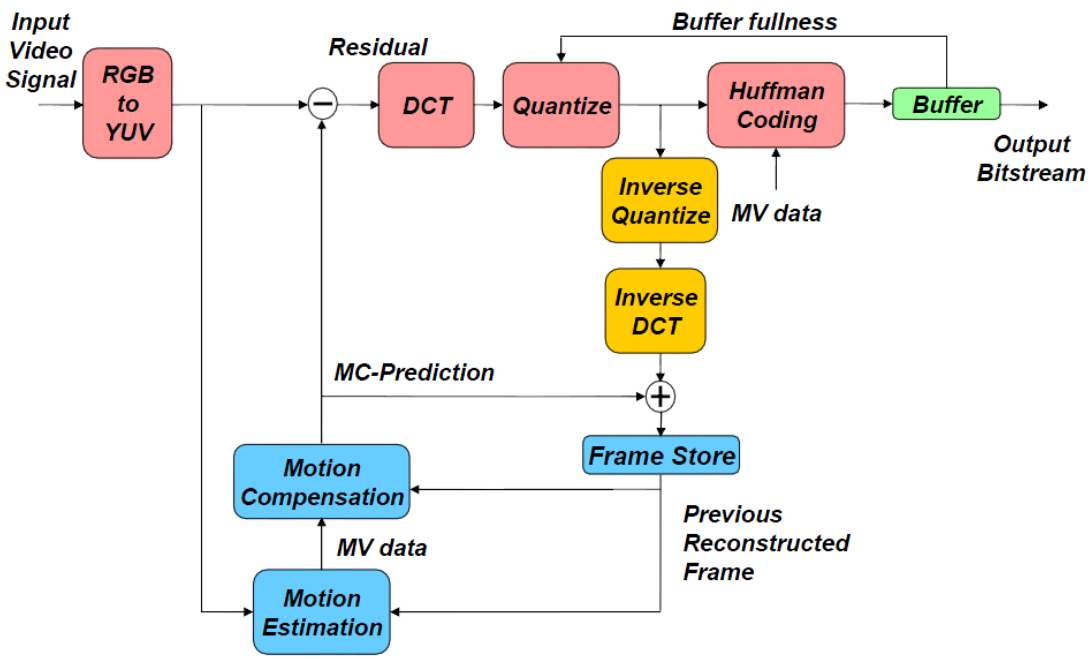
\includegraphics[width=\linewidth]{encoder.png}
\end{center}

The corresponding decoder then looks like this:
\begin{center}
	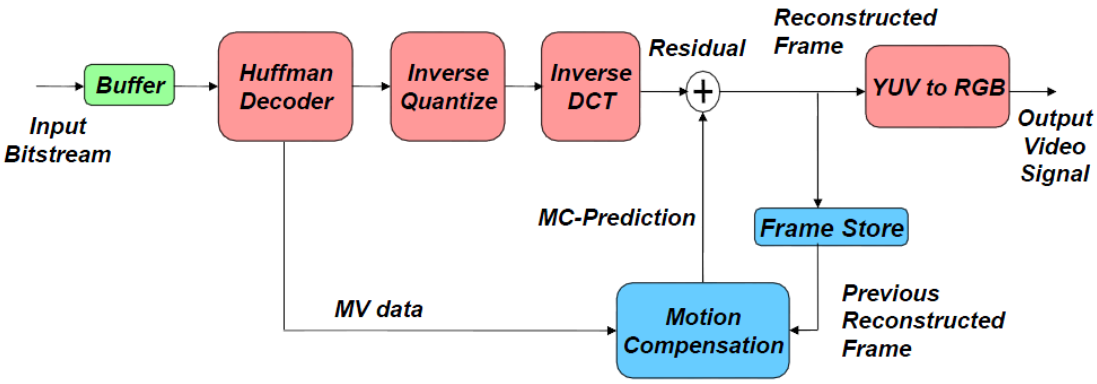
\includegraphics[width=\linewidth]{decoder.png}
\end{center}